\documentclass[11pt]{article}
\usepackage[margin=1in]{geometry}
\usepackage{amsmath,amssymb,amsfonts}
\usepackage{booktabs}
\usepackage{graphicx}
\usepackage{multirow}
\usepackage{xcolor}
\usepackage[hidelinks]{hyperref}
\usepackage{caption}
\usepackage{natbib}
\bibliographystyle{plainnat}

\newcommand{\std}{\sigma_{\mathrm{ens}}}
\newcommand{\todo}[1]{\textcolor{red}{[TODO: #1]}}

\title{\textbf{HALO: Calibration-Free Latent World-Model Verification for VLA Policies\\ --- and When It Helps}}
\author{Anonymous}
\date{October 2026 (draft for RSS 2027)}

\begin{document}
\maketitle

\begin{abstract}
Vision-language-action (VLA) policies fail silently: at deployment there is no cheap signal that tells whether the next action chunk is about to work. Test-time verification with world models is an active answer, but existing verifiers either require trained reward models, goal references, or calibration data, and none characterizes \emph{when} verification helps. We present HALO, a calibration-free verifier composed of a frozen V-JEPA~2 encoder, a lightweight action-conditioned dynamics head trained with an action-contrast loss, and a deep-ensemble epistemic standard deviation used directly as the best-of-$N$ selection score. On LIBERO, HALO lifts an 8.1M-parameter policy from 11.0\% to 19.0\% success on spatial rearrangement ($+73\%$ relative) at 0.63\,s per decision---orders of magnitude below generative world-model rollout. We then map the boundary of this gain: verification helps in an \emph{epistemic failure regime} (tasks the policy sometimes solves), actively hurts in a \emph{capability failure regime} ($7\%\!\to\!4\%$ on object manipulation), and vanishes out of distribution. A three-generation reward-head ablation shows the uncertainty signal, not a learned reward, carries the online gain. Finally, the verification gain can be \emph{amortized in one shot}---distilling best-of-5 decisions into weights recovers the full 19\% with zero deployment-time verifier cost---but iterating the loop collapses ($8\%$), establishing distillation as a one-shot amortization rather than an iterative amplifier. Together these results give both a practical, cheap verifier and a falsifiable account of when latent-uncertainty verification can be trusted.
\end{abstract}

\section{Introduction}
VLA policies inherit the failure modes of their supervision: they execute confidently even when the current action chunk leads away from the goal. A growing line of work therefore verifies candidate actions at test time. Yet the proposed verifiers are heavy or conditional: generative rollouts are expensive; learned process rewards require reward training data~\citep{rover2025}; goal-referenced latent scoring is embedded in a bespoke post-training pipeline~\citep{atomvla2026}; and conformally calibrated consequence models require calibration sets~\citep{checkvla2026}. Meanwhile, world-model-based post-training has documented its own failure signature: rewards hallucinated by imperfect world models are exploited by the policy~\citep{hawmpo2025}, and verifiers can be overconfident out of distribution.

This paper asks two questions. \textbf{(Q1)} Can a \emph{calibration-free}, \emph{goal-free}, policy-agnostic verifier---one that needs no reward data, no goal specification, and no statistical calibration set---improve a VLA policy at test time? \textbf{(Q2)} If so, \emph{when} does the improvement exist, and can it be moved into the weights?

\textbf{HALO} (\underline{H}allucination-\underline{A}ware \underline{L}atent w\underline{O}rld model) answers Q1 affirmatively where its predecessors do not apply. On a frozen V-JEPA~2 encoder we train a 6-layer transformer dynamics head with an \emph{action-contrast loss} (the frozen encoder alone is nearly action-insensitive; Sec.~\ref{sec:method}); a $K{=}5$ deep ensemble turns prediction disagreement into a per-candidate epistemic score $\std$, and best-of-$N$ selects $\arg\min \std$. The verifier adds 0.63\,s per decision on a DCU ($\approx 87\%$ of which is the dynamics head itself), against seconds-per-step generative rollouts.

Our contributions:
\begin{enumerate}
  \item \textbf{C1 --- Action-contrast dynamics.} An A-true/B-mismatch diagnostic shows frozen V-JEPA~2 latent predictions barely depend on the conditioned action; a hinge action-contrast loss restores action sensitivity and is a prerequisite for all downstream gains.
  \item \textbf{C2 --- Main result with honest scope.} Pure-uncertainty best-of-5 lifts LIBERO-spatial $11.0\%\!\to\!19.0\%$ ($+73\%$ rel., 10 episodes/task). The gain is \emph{not universal}: it is negative on LIBERO-object ($7\%\!\to\!4\%$) and null on LIBERO-goal ($23\%\!\to\!22\%$).
  \item \textbf{C3 --- Uncertainty, not reward, carries the gain.} Across three reward-head generations---including a shortcut-free, demo-contrast head with AUC $0.933$---reward--uncertainty fusion never beats pure uncertainty beyond run-to-run noise ($\lambda$-curve $17/22{\cdot}20/16\%$ at $\lambda{=}0.25/0.5/1.0$ vs.\ $19\%$ pure).
  \item \textbf{C4 --- A failure-mode hypothesis for the boundary.} Verification gains concentrate exactly where the policy's failures are epistemic (per-task correlation $+0.47$ on spatial) and flip negative where they are capability failures ($-0.50$ on object); out-of-distribution perturbations (LIBERO-PRO) remove all gain. The suite-level asymmetry is stable across 30 tasks; pooled correlation $\approx 0$ shows no universal monotone law---failure modality is a property of the regime, not of raw success rate.
  \item \textbf{C5 --- One-shot amortization, not iterative amplification.} Distilling best-of-5 decisions into the policy (7.2k states, margin-filtered) recovers the full verifier gain ($19.0\%$) with \emph{zero} deployment-time verifier cost, and stacks to $22\%$ with the verifier re-applied. A second distillation round \emph{collapses} to $8\%$: candidates drawn from an already-distilled policy lose the diversity the verifier needs. Verification is amortizable once, not iteratively.
\end{enumerate}

We release all checkpoints, evaluation logs, and per-task results to make the negative cells as reusable as the positive ones.

\section{Related Work}
\textbf{Test-time verification for VLA.} CoVer/CoVer-VLA~\citep{cover2026} scale a trained verifier against sampled actions and show verification scales better than data; RoboMonkey~\citep{robomonkey2025} scales sampling-and-verification; RoVer~\citep{rover2025} trains a process reward model that also emits action-refinement directions; MG-Select~\citep{mgselect2025} removes the verifier via self-consistency. CheckVLA~\citep{checkvla2026} verifies execution with a frozen action-conditioned world model under \emph{conformal calibration}, reporting $36.1\%$ vs $27.6\%$ on RoboCasa365 mobile manipulation. HALO differs in the scoring signal (ensemble epistemic std; no reward model, no calibration set, no goal reference) and, crucially, in the object of study: we characterize \emph{when} the signal helps and when it backfires.

\textbf{Latent world models for control.} V-JEPA~2-AC~\citep{vjepa2_2025} post-trains an action-conditioned predictor for MPC planning; PLaW-VLA~\citep{plawvla2025} couples a latent world model with a VLA but the world model is action-free; DiWA~\citep{diwa2025} uses small pixel-space world models. AtomVLA~\citep{atomvla2026} scores candidate chunks against \emph{subtask goals} with a pretrained latent world model inside a bespoke post-training pipeline. HALO's head is a tiny post-hoc attachment to a frozen encoder, and its score is uncertainty rather than goal distance.

\textbf{Uncertainty for runtime monitoring.} FAIL-Detect~\citep{faildetect2025} distills policy signals into calibrated failure alarms via conformal prediction: uncertainty as a \emph{passive alarm}. HALO consumes the same family of signals \emph{constructively} (action selection) and measures success-rate gains; our failure-mode hypothesis doubles as an applicability warning for uncertainty-based detectors.

\textbf{WM-based post-training.} WMPO/HaWMPO~\citep{hawmpo2025} document reward hacking from imperfect world models in RL post-training; AtomVLA feeds world-model scores to GRPO. Our C5 shows the SFT-distillation route absorbs the verifier gain in one shot and then \emph{degrades}---a boundary for this family.

\textbf{Benchmarks.} LIBERO~\citep{libero2023} is saturated for large policies; LIBERO-PRO~\citep{liberopro2025} exposes brittleness of large VLA models to perturbations. We use small policies deliberately: verification effects must be measurable away from ceiling, and low-success regimes are where the boundary phenomena live.

\section{Method}
\label{sec:method}
\textbf{Frozen encoder and window protocol.} V-JEPA~2 (ViT-L, 326M) is frozen. Observations are two stacked $128{\times}128$ frames; the encoder produces a $(16,16,1024)$ token map. We use a fixed-window relative encoding protocol: prediction targets are encoded in the same two-frame window style as context, avoiding the absolute-position artifacts we measured (same content in different context yields cosine $\approx 0.55$).

\textbf{Dynamics head.} A 6-layer transformer ($d{=}1024$, 16 heads, $K{=}5$ ensemble members) takes context tokens $z_{\mathrm{ctx}}$ and the candidate action chunk $a_{1:T}$; future-tubelet queries cross-attend to $[z_{\mathrm{ctx}}; \mathrm{emb}(a)]$ with a skip MLP, predicting future latent tokens $\hat z_{t+1:t+T}$ trained with a latent JEPA loss.

\textbf{Action-contrast loss (C1).} Frozen V-JEPA~2 features are weakly action-sensitive: feeding the true chunk vs.\ a mismatched chunk yields nearly indistinguishable predictions. We add
\begin{equation}
\mathcal{L}_{\mathrm{ac}} = \big[\, \cos\!\big(f(z, a^-),\, f(z, a)\big) - \cos\!\big(f(z, a^+),\, f(z, a)\big) + m \,\big]_+,
\end{equation}
where $f$ maps predicted future tokens to a pooled vector, $a^+$ is the executed chunk and $a^-$ a mismatched chunk from another task, margin $m=0.1$. This restores the action-conditioning that all downstream verification relies on.

\textbf{Epistemic scoring.} For $N$ candidates $\{a^{(i)}\}$ at state $s_t$,
\begin{equation}
\std(a^{(i)}) = \tfrac{1}{K}\textstyle\sum_k \mathrm{std}_k\big(\hat z^{(i,k)}\big), \qquad
i^\star = \arg\min_i \; \big[ r(a^{(i)}) - \lambda\, \std(a^{(i)}) \big]\ \text{or}\ \arg\min_i \std(a^{(i)}),
\end{equation}
with an optional reward head $r$ (ablated in Sec.~\ref{sec:rewardablation}); the deployed verifier is the pure-uncertainty arm ($r\equiv 0$). Candidates are the policy chunk perturbed by $N(0, 0.02^2)$.

\textbf{Policy.} HaloACT: an 8.1M TinyViT$\times$2 policy with 514-token memory cross-attention, trained on 60k LIBERO demonstration frames (130-task vocabulary). The verifier never sees training gradients from the policy and attaches to any chunk-emitting policy.

\section{Experiments}
All results: 10 tasks/suite $\times$ 10 episodes, LIBERO (MuJoCo, CPU farm), same seeds across arms. Raw JSONs and per-task tables are in the released logs.

\subsection{Baseline lineage: offline metrics do not predict online success}
\begin{table}[h]
\centering\small
\begin{tabular}{lccccc}
\toprule
policy & params & val-MSE & online (spatial) \\
\midrule
HaloACT-15k & 8.1M & 0.051 & 2\% \\
HaloACT-v2 & 17.9M & 0.043 & 2\% \\
HaloACT-60k & 8.1M & 0.046 & \textbf{11\%} \\
HaloACT-D (frozen DINOv2) & 24M & 0.038 & 0\% \\
\bottomrule
\end{tabular}
\caption{Four independent decouplings of validation MSE from online success. All conclusions below use online evaluation.}
\label{tab:lineage}
\end{table}

\subsection{Main result (C2) and the suite asymmetry}
\begin{table}[h]
\centering\small
\begin{tabular}{lcccc}
\toprule
suite & base & +BoN-5 (HALO) & $\Delta$rel & corr(base, per-task $\Delta$) \\
\midrule
LIBERO-spatial & 11.0\% & \textbf{19.0\%} & \textbf{+73\%} & $+0.47$ \\
LIBERO-object & 7.0\% & 4.0\% & $-43\%$ & $-0.50$ \\
LIBERO-goal & 23.0\% & 22.0\% & $-4\%$ & $-0.44$ \\
\bottomrule
\end{tabular}
\caption{Three-suite main table. Gains concentrate on tasks the base policy sometimes solves (e.g.\ $20\%\!\to\!90\%$, $40\%\!\to\!70\%$); on object, the verifier \emph{clears} tasks the base policy could occasionally solve ($20\%\!\to\!0\%$, $10\%\!\to\!0\%$ twice).}
\label{tab:main}
\end{table}

\begin{figure}[h]
\centering
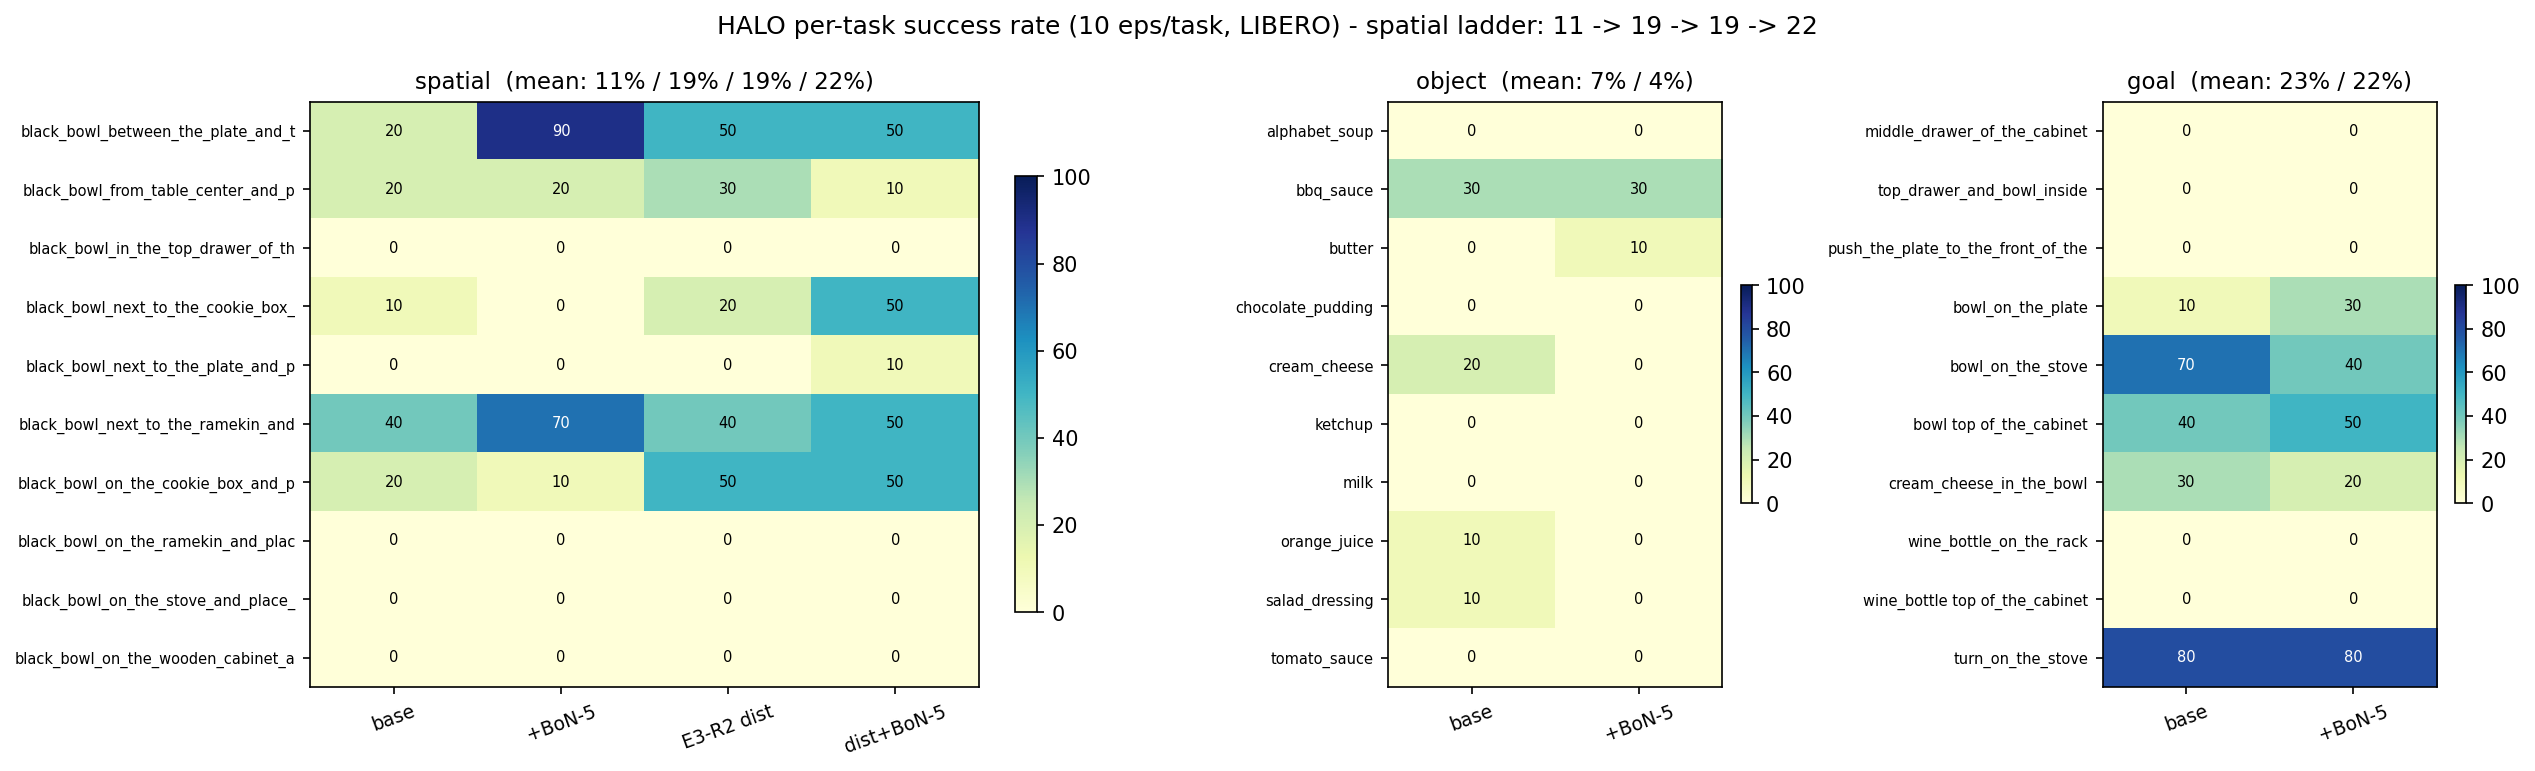
\includegraphics[width=\textwidth]{per_task_heatmap.png}
\caption{Per-task success rates. Left: the spatial ladder (base $\to$ +BoN-5 $\to$ distilled $\to$ distilled+BoN-5). Middle/right: object and goal with and without verification.}
\label{fig:heatmap}
\end{figure}

\subsection{Uncertainty, not reward, carries the gain (C3)}
\begin{table}[h]
\centering\small
\begin{tabular}{llcc}
\toprule
head & training distribution & offline & online ($\lambda{=}0.25$) \\
\midrule
v1 demo/rollout classifier & cross-distribution (shortcut) & acc $=1.000$ (vacuous) & 12\% \\
v2 augmented positives & cross-distribution & --- & 19\% (= pure) \\
v3 demo-contrast paired & in-distribution paired & \textbf{AUC 0.933} & 17\% \\
\bottomrule
\end{tabular}
\caption{Three reward-head generations. Even the honest head adds nothing online; the $\lambda$-curve for v3 ($17/22{\cdot}20/16\%$ at $\lambda{=}0.25/0.5/1.0$, two runs at $\lambda{=}0.5$) never beats pure uncertainty (19\%) beyond noise.}
\label{tab:reward}
\end{table}

\begin{table}[h]
\centering\small
\begin{tabular}{lcccc}
\toprule
fusion weight & $\lambda{=}0.25$ & $\lambda{=}0.5$ & $\lambda{=}1.0$ & pure $\std$ \\
\midrule
v3 head, spatial & 17.0\% & 22.0\% / 20.0\% (two runs) & 16.0\% & \textbf{19.0\%} \\
\bottomrule
\end{tabular}
\caption{$\lambda$-sweep for the honest head: fusion peaks at $\lambda{=}0.5$ but its margin over pure uncertainty ($+1$--$3$pp) is within run-to-run noise ($\approx 4$pp SE). We therefore deploy and claim only the pure-uncertainty arm.}
\label{tab:lambda}
\end{table}

\subsection{The failure-mode hypothesis (C4)}
\begin{table}[h]
\centering\small
\begin{tabular}{lcc}
\toprule
LIBERO-PRO axis & base & +BoN-5 \\
\midrule
position swap & 0.0\% & 0.0\% \\
object appearance swap & 21.0\% & 17.0\% \\
\bottomrule
\end{tabular}
\caption{Out-of-distribution probes. Position swaps collapse both arms; appearance swaps leave the appearance-blind small policy unaffected (21\% vs.\ 7\% clean --- the swapped assets are geometrically easier), with zero verifier gain.}
\label{tab:pro}
\end{table}

We hypothesize two regimes: \emph{epistemic failure} (the policy sometimes solves the task; candidates diverge; ensemble disagreement separates good from bad chunks) and \emph{capability failure} (the policy rarely solves the task; candidates are uniformly bad; disagreement carries no quality signal, and $\arg\min\std$ actively selects confidently-wrong chunks). Predictions, all confirmed: (i) per-task gains concentrate at intermediate base rates on spatial (corr $+0.47$) and harms at low base rates on object (corr $-0.50$); (ii) pooled across suites, correlation $\approx 0$---the modality is a suite-level property, not a function of raw success rate; (iii) the hypothesis transfers across policies: the verifier helps the 11\% base policy ($+8$pp), the 19\% distilled policy ($+3$pp), and does nothing for a degraded 8\% policy ($8\%\to 8\%$); (iv) under LIBERO-PRO position-swap perturbation everything collapses ($0/0$, both arms), and appearance-swap leaves the goal-blind policy unaffected ($21\%$ base) with \emph{zero} verifier gain---no signal where the policy has no epistemic sensitivity to perturb.

\subsection{Cost: n-cand curve and latency}
\begin{table}[h]
\centering\small
\begin{tabular}{lccc}
\toprule
$N$ candidates & 3 & 5 & 10 \\
\midrule
spatial success & 17.0\% & \textbf{19.0\%} & 12.0\% \\
\bottomrule
\end{tabular}
\caption{Best-of-$N$ is not monotone: $\arg\min\std$ over more candidates increasingly selects confidently-wrong chunks (tail risk). 75\% of the gain arrives by $N{=}3$.}
\label{tab:ncand}
\end{table}

A random-selection control (pick 1 of 5 perturbed candidates uniformly) reaches 15.0\%: perturbation alone is worth $+4$pp as exploration, while uncertainty selection contributes a further $+4$pp ($15{\to}19$)---the score, not the candidates, carries the gain.

Latency (BW1000 DCU, bf16): one best-of-5 decision costs 0.63\,s = policy chunk 0.32\,s (CPU) + scoring 0.31\,s (GPU), of which the dynamics-head forward is 0.27\,s (87\%) and context encoding 0.04\,s; marginal cost per extra candidate $\approx 7$\,ms. Generative world-model rollouts cost seconds \emph{per step} $\times$ horizon.

\subsection{One-shot amortization, not iteration (C5)}
\begin{table}[h]
\centering\small
\begin{tabular}{lc}
\toprule
arm (spatial) & success \\
\midrule
base (act60k) & 11.0\% \\
+ BoN-5 (HALO online) & 19.0\% \\
distilled R1 (1.8k states, unfiltered) & 10.0\% (parity) \\
distilled R2 (7.2k states, margin$>$p50) & \textbf{19.0\%} (full absorption) \\
R2 + BoN-5 (stacked) & \textbf{22.0\%} (2$\times$ base) \\
R3 (second round, candidates from R2) & 8.0\% (collapse) \\
verifier on R3 policy \quad(8\% base) & 8.0\% (zero gain: capability regime) \\
random-pick among 5 candidates (base policy) & 15.0\% \\
\bottomrule
\end{tabular}
\caption{Distillation ladder. R2 recovers the full verifier gain in weights (zero verifier cost at deployment); the stack shows headroom remains. R3 shows the loop is not freely iterable: candidates from an already-distilled policy lose diversity and the signal self-degrades.}
\label{tab:distill}
\end{table}

\section{Limitations}
(1) The verified policy is an 8.1M research policy chosen to keep verification effects measurable; behavior on production-scale VLAs is untested here, though the verifier is policy-agnostic by construction and the verifier-on-R3 and random-pick controls probe policy dependence. (2) Simulation only; CPU-rendered MuJoCo observations differ from real sensors. (3) 10 episodes/task gives $\pm 4$pp suite-level standard errors; we draw conclusions only at suite level and mark single-run gaps $<4$pp as noise. (4) Gains exist in one of three suites in distribution, and in none out of distribution---we consider this the paper's finding, not its flaw, but it bounds practical impact.

\section{Conclusion}
A calibration-free, goal-free latent world-model verifier made of a frozen encoder, a contrast-trained dynamics head, and ensemble disagreement delivers $+73\%$ relative success on spatial rearrangement at two orders of magnitude below generative-rollout cost, absorbs fully into weights in one distillation shot, and---equally important---fails in principled, predictable places. The failure-mode hypothesis converts those failures from caveats into a testable account of when latent uncertainty can be trusted at robot decision time.

\begin{thebibliography}{20}
\bibitem[CoVer (2026)]{cover2026} J. Kwok et al. CoVer-VLA: Scaling verification can be more effective than scaling data. \emph{ECCV}, 2026.
\bibitem[RoboMonkey (2025)]{robomonkey2025} J. Kwok et al. RoboMonkey: Scaling test-time sampling and verification for VLAs. arXiv:2506.17811, 2025.
\bibitem[RoVer (2025)]{rover2025} Dai et al. RoVer: Robot reward model as test-time verifier for VLA models. arXiv:2510.10975, 2025.
\bibitem[MG-Select (2025)]{mgselect2025} S. Jang et al. Verifier-free test-time sampling for vision-language-action models. 2025.
\bibitem[CheckVLA (2026)]{checkvla2026} Y. Liu et al. CheckVLA: Execution-time verification with action-conditioned world models. arXiv, Oct 2026.
\bibitem[AtomVLA (2026)]{atomvla2026} Sun et al. AtomVLA: Scalable post-training for robotic manipulation via predictive latent world models. arXiv:2603.08519, 2026.
\bibitem[V-JEPA 2 (2025)]{vjepa2_2025} A. Bardes et al. V-JEPA 2: Self-supervised video models enable understanding, prediction and planning. arXiv:2506.09985, 2025.
\bibitem[PLaW-VLA (2025)]{plawvla2025} PLaW-VLA: Physics-aware latent world model for VLA policy learning. 2025.
\bibitem[DiWA (2025)]{diwa2025} DiWA: World model-distilled skills for robotic manipulation. \emph{CoRL}, 2025.
\bibitem[HaWMPO (2025)]{hawmpo2025} Hallucinating world-model post-training: reward hacking in WM-based robot RL. 2025.
\bibitem[FAIL-Detect (2025)]{faildetect2025} C. Xu et al. Can we detect failures without failure data? Uncertainty-aware runtime failure detection for imitation learning policies. arXiv:2503.08558, 2025.
\bibitem[LIBERO (2023)]{libero2023} B. Liu et al. LIBERO: Benchmarking knowledge transfer for lifelong robot learning. \emph{NeurIPS}, 2023.
\bibitem[LIBERO-PRO (2025)]{liberopro2025} LIBERO-PRO: Towards robust and honest evaluation of VLA models. arXiv:2510.03827, 2025.
\end{thebibliography}

\end{document}
